\documentclass[]{article}
\usepackage{hanging}
\usepackage{graphicx}
\usepackage{geometry}
\usepackage{caption}
\usepackage{float}
\usepackage{url}

\captionsetup[figure]{labelfont=it, labelsep=period}

\geometry{left=2cm, right=2cm}

\title{
  Accuracy of Machine Learning Methods in Predicting Diabetes \\
  \vspace{5mm}
  \large GitHub Repository: https://github.com/alexz957unc/COMP-562-Final-Project}
\author{Alexander Zheng\and Connor Morin\and Jingyu Li\and Yibo Wang}
\date{April 30, 2024}

\begin{document}

\maketitle

\section{Introduction}
Diabetes is a chronic disease that affects insulin, a hormone responsible for keeping blood sugar at healthy levels, and it causes the body to either not produce insulin or not respond to it well (CDC, 2023b). The cost and seriousness of diabetes in the U.S. is not to be understated. According to the National Diabetes Statistics Report, 38.4 million people in the U.S. have diabetes, diagnosed or undiagnosed, which is over 11 percent of the total population. Furthermore, 97.6 million people have prediabetes, which is a staggering 30 percent of the U.S. population (CDC, 2023c). A 2022 study from the National Library of Medicine estimated the total cost of diabetes to be nearly \$413 billion in both direct medical costs and indirect costs (Parker et al., 2024). Unfortunately, the consequences from such statistics are dire. In 2021, the eighth leading cause of death in the U.S. was diabetes, with 399,401 death certificates listing diabetes as either an underlying or contributing cause of death (CDC, 2023c). However, it is not all bad news; once an individual learns they have diabetes, certain measures can be taken to mitigate the risks associated with the disease and possibly prevent it altogether.

This notion leads us to some questions that we believe machine learning methods may be particularly useful in answering. If we know that diabetes can be mitigated or prevented, then can we use ML methods to identify particular risk factors associated with diabetes, and can any of these methods make accurate predictions on if an individual has diabetes? If so, which ML methods are the best and most accurate for doing so? Being able to answer such questions could be the key to helping identify cases of undiagnosed diabetes or individuals that are in danger of developing it so that they can begin to take measures to mitigate or reverse their condition as soon as possible. These are the questions we look to explore in this analysis.

\subsection{Dataset}
To conduct our analysis, we will be using data from the CDC's Behavioral Risk Factor Surveillance System (BRFSS), which completes yearly telephone surveys for over 400,000 Americans, collecting data about "health-related risk behaviors and events, chronic health conditions, and use of preventive services" (CDC, 2014). The particular dataset we will be using is from a BRFSS survey in 2015, and it contains 70,692 responses and 21 feature variables for each. A response corresponds to an individual with either no diabetes, represented with a "0," or prediabetes or diabetes, represented with a "1," and the dataset contains an even split of responses with no diabetes and prediabetes/diabetes.

\section{Approach}
Our goal is to predict a binary outcome (to be more specific, whether someone has diabetes) using several machine learning classification models. The dataset we used includes multiple features that could potentially influence the prediction outcome. We have done some processing, such as  encoding categorical variables and splitting the dataset into training and test datasets (80-20 split).

\subsection{Logistic Regression}
First, a logistic regression model was set up to perform up to 2000 iterations. It was provided with two sets of data for training and testing. Its effectiveness was evaluated using F1, accuracy, precision, and recall scores to address any class imbalances. Additionally, the influence of each feature on the model’s decisions was produced.

\subsection{Decision Tree Classifier}
Next, using a decision tree classifier optimized by a grid search with 5-fold cross-validation, we determined the best set of hyperparameters. Specifically, we identified the maximum depth of the tree, the minimum number of samples required to split an internal node, and the minimum number of samples required to be at a leaf node. The optimal values we found were a maximum depth of 8, with a minimum of 1 leaf sample and 10 samples required to split a node. The model's performance was then evaluated on the same metrics as above, and feature influences were again examined.

\subsection{Random Forest}
Third, we used a random forest model. In this random forest model, we again conducted hyperparameter tuning using grid search and 5-fold cross-validation to optimize the model's performance. As a result, we set the maximum depth of each tree in the forest to be 12, the n-estimator to 200, and the random states to 42. After the model was run, standard performance metrics were used to assess its robustness, and the most important features were studied.

\subsection{KNN}
Next, we attempted to classify the data with a k-nearest neighbors classifier. The number of neighbors used was determined by taking the square root of the number of total samples. The KNN model utilized 265 neighbors for the classification. After being trained on the training data, this model underwent performance evaluation using F1 score, accuracy, precision, and recall. Note that feature importance could not be produced for the KNN model, so it was not as helpful in answering questions about the impact of different features.

\subsection{SVM}
The fifth method we used is the SVM. The SVM used a linear kernel with a regularization parameter of 1.0. The model's performance was also assessed using F1 score, accuracy, precision, and recall. An analysis was also performed to investigate the feature importance.

\subsection{XGBoost}
We did a fair amount of hyperparameter tuning for XGBoost, carefully varying the learning rate, tree depth, number of trees in the ensemble, and regularization terms. We found that the optimal parameters were identified as a learning rate of 0.1, 200 estimators, and regularization terms reg\_alpha at 0.5 and reg\_lambda at 1. The model was then evaluated using the standard set of metrics, and feature importance was visually represented to highlight the most influential predictors.

\subsection{AdaBoost}
Finally, the AdaBoost classifier underwent hyperparameter tuning using grid search to optimize key parameters. After identifying the optimal settings, the model was trained and evaluated on the test set using the same performance metrics. We also investigated the resulting feature importance of the AdaBoost classification. 

\section{Conclusion}
The combined accuracy of all models ranges from 0.72558 to 0.75536. AdaBoost surpasses other models in terms of both accuracy (0.75536) and F1 score (0.75502), making it the most compelling model in estimating diabetes. Its high-rate precision (0.75694) and recall (0.75536) indicate a balanced performance, which is essential for practical applications in the medical field. Despite AdaBoost's immensely competitive success, Random Forest and XGBoost also show respectable results, with XGBoost reaching the second highest F1 score. This suggests that ensemble methods, in general, are more effective for this application due to their ability to handle complex patterns and data imbalances better than simpler models like Logistic Regression. Likewise, KNN provided the worst results as this method performs poorly with a large number of features.
\begin{figure}[h]
  \centering
  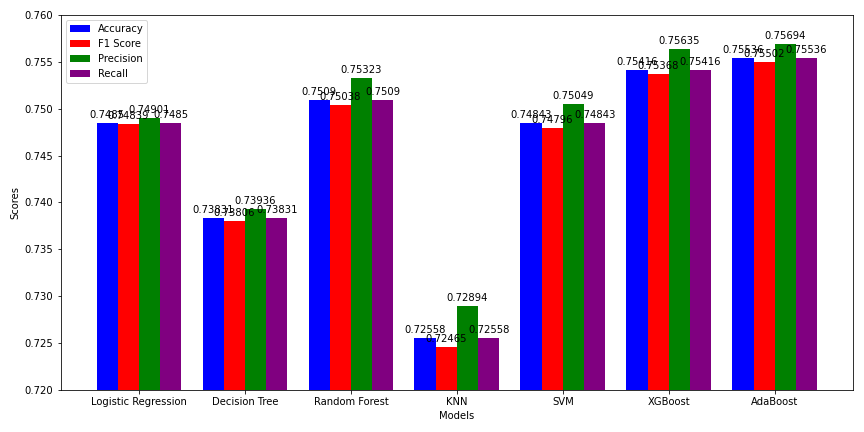
\includegraphics[width=0.8\textwidth]{combined.png}
  \caption{Accuracy, F1, precision, and recall values for each model}
  \label{fig:bar}
\end{figure}
While measurements indicate that AdaBoost is the most accurate and has the highest F1 score, the overall model misclassification error does not vary greatly or is very similar across all models. This suggests that improvements in model performance may also be obtained from further feature engineering or data preprocessing to reduce these errors. It is worth noting that the two boosting methods perform better than other methods. 

The reason why boosting methods like AdaBoost and XGBoost often perform better, particularly in complex predictive tasks like diabetes prediction from survey data, can be attributed to several key characteristics of boosting algorithms. First, many traditional models like decision trees tend to overfit the data, showing high variance but low bias, whereas models like logistic regression may underfit, showing high bias but low variance. Boosting methods manage to balance bias and variance effectively. They build on top of weak models (typically high bias) and by focusing iteratively on reducing errors, they also manage to keep variance in check. Also, Boosting is designed to sequentially correct the mistakes of prior models and combine many weak learners (models that perform only slightly better than random guessing) to create a strong learner (Chen \& Guestrin, 2016).

This approach effectively reduces both the bias (error due to erroneous assumptions in the learning algorithm) and variance (error from sensitivity to small fluctuations in the training set) of the model. In addition, according to Hastie et al. (2009) and Murphy (2012), boosting methods can naturally process continuous and classified data and can naturally process missing data. 

\subsection{Results and Analysis}
Examining the outcome with the two models that have the highest accuracy scores, we utilized feature importance plots from both the AdaBoost and XGBoost models to derive multiple inferences about the importance of different predictors in determining the likelihood of someone being diagnosed with diabetes.
\begin{figure}[h]
  \centering
  \begin{minipage}[b]{0.45\textwidth}
    \centering
    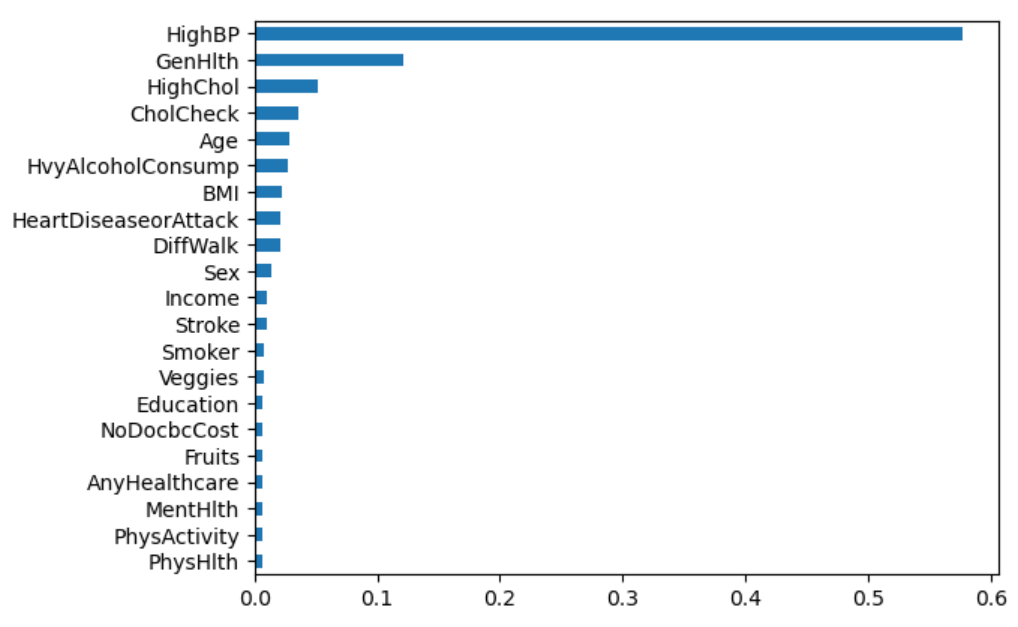
\includegraphics[width=0.8\linewidth]{xgboost_w.png}
    \caption{XGBoost feature importance}
  \end{minipage}\hfill
  \begin{minipage}[b]{0.45\textwidth}
    \centering
    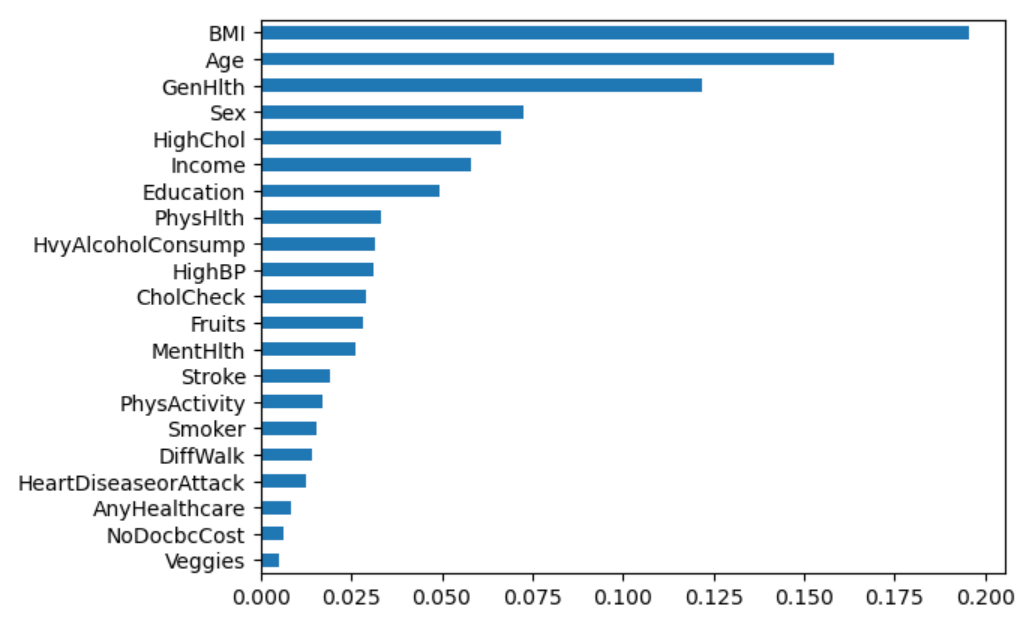
\includegraphics[width=0.8\linewidth]{adaboost_w.png}
    \caption{AdaBoost feature importance}
  \end{minipage}
\end{figure}
In the XGBoost model, high blood pressure (HighBP) is the most influential variable,
indicating a strong association with diabetes. This factor is still important in the AdaBoost model but ranks slightly lower. 

The AdaBoost models, which place an emphasis on sex and body mass index as well as on their interactions, show the prediction that obesity and increased body mass index are strong predictors of increased diabetes risk. The AdaBoost model therefore revealed that these two factors markedly influence diabetes risk and that by looking at sex as well as body mass index, their combined effect on diabetes risk is certainly not simply additive.

The two models each individually and consistently identify Cholesterol Levels (HighChol) as well as General Health (GenHlth) as a factor for prediction. However, their orders of importance are different. This underscores the significance of lifestyle factors in diabetes risk, and Age shows up to be a significant factor in both models, as it should be since diabetes risk grows exponentially with age.
\pagebreak

\section{References}
\begin{hangparas}{.25in}{1}
Centers for Disease Control and Prevention. (2014, May 16). \textit{CDC - about BRFSS}. Centers for Disease Control and Prevention. \url{https://www.cdc.gov/brfss/about/index.htm} \\

Centers for Disease Control and Prevention. (2023a, May 8). \textit{Chronic disease center (NCCDPHP)}. Centers for Disease Control and Prevention. \url{https://www.cdc.gov/chronicdisease/index.htm} \\

Centers for Disease Control and Prevention. (2023b, September 5). \textit{What is diabetes?}. Centers for Disease Control and Prevention. \url{https://www.cdc.gov/diabetes/basics/diabetes.html} \\

Centers for Disease Control and Prevention. (2023c, November 29). \textit{National Diabetes Statistics Report}. Centers for Disease Control and Prevention. \url{https://www.cdc.gov/diabetes/data/statistics-report/index.html} \\

Chen, T. and Guestrin, C. (2016). Xgboost: A scalable tree boosting system. In Proceedings of the 22Nd ACM SIGKDD International Conference on Knowledge Discovery and Data Mining, KDD 16, pages 785–794, New York, NY, USA. \\

Hastie, T., Tibshirani, R., and Friedman, J. (2009). The Elements of Statistical Learning: Data Mining, Inference, and Prediction, Second Edition. Springer Series in Statistics. Springer. \\

Murphy, K. P. (2012). Machine Learning: A Probabilistic Perspective. The MIT Press. \\

Parker, E. D., Lin, J., Mahoney, T., Ume, N., Yang, G., Gabbay, R. A., ElSayed, N. A., \& Bannuru, R. R. (2024). Economic Costs of Diabetes in the U.S. in 2022. \textit{Diabetes care}, 47(1), 26–43. \url{https://doi.org/10.2337/dci23-0085} \\
\end{hangparas}

\end{document}